\documentclass[12pt,twoside]{report}

% PACCHETTI FONDAMENTALI
\usepackage{amsmath,amsfonts,amssymb,amsthm, dsfont, mathtools}
\usepackage{graphicx}
\usepackage[a4paper,outer=2cm,inner=3cm,top=3.3cm,bottom=2.5cm]{geometry}
\usepackage{float} % per il comando [H] per le tabelle
\usepackage{enumerate} % per scegliere i caratteri degli elechi
\usepackage{accents}
\usepackage{esint}
% intestazione pagine
\usepackage{fancyhdr}

% NOMENCLATURA
% indice
\renewcommand*\contentsname{Indice}
% capitoli
\renewcommand{\chaptername}{Capitolo}
% appendici
\renewcommand{\appendixname}{Appendice}
% bibliografia
\renewcommand\bibname{Bibliografia}
    
% TITOLI
% per mettere i titoli dei capitoli sulla destra e aggiungere una riga di separazione sotto
\usepackage{titlesec} 
\newcommand*{\justifyheading}{\raggedleft}
\titleformat{\chapter}[display]
  {\normalfont\LARGE\bfseries\justifyheading}
  {\chaptertitlename\ \thechapter \vspace*{-0.5cm}}
  {20pt}{\Huge}
  [\vspace*{0.3cm}\hrule height 0.08cm \vspace*{1cm}]

% STUTTURE FONDAMENTALI
% teoremi
\theoremstyle{plain}
\newtheorem{theorem}{Teorema}[section]
% lemmi
\newtheorem{lemma}[theorem]{Lemma}
% teoremi con nomi
\newtheoremstyle{named}{}{}{\itshape}{}{\bfseries}{.}{.5em}{\thmnote{#3} #2}
\theoremstyle{named}
\newtheorem{namedtheorem}[theorem]{Teorema}
% ipotesi
\newenvironment{ipotesi}%
{\quad\left|\quad\def\arraystretch{1.2}\begin{array}{@{}l@{}}}%
{\end{array}\right.}
% tesi
\newcommand{\tesi}[1]{\quad\left|\quad{#1}\right.}
% unico comando per ipotesi e tesi
\newcommand{\hpth}[2]
{
\begin{flalign*}
\quad\quad\quad
\text{Ipotesi}
&\begin{ipotesi}
#1
\end{ipotesi}&&\\
\quad\quad\quad
\text{Tesi}
&\tesi{#2}&&
\end{flalign*}
}
% quando ci sono 2 tesi distinte
\newcommand{\hpthth}[3]
{
\begin{flalign*}
\quad\quad\quad
\text{Ipotesi}
&\begin{ipotesi} 
#1
\end{ipotesi}&&\\
\quad\quad\quad
\text{Tesi 1}
&\tesi{#2}&&\\
\quad\quad\quad
\text{Tesi 2}
&\tesi{#3}&&
\end{flalign*}
}
% dimostrazioni
\renewcommand*{\proofname}{\bf{Dimostrazione:}}
\renewcommand\qedsymbol{\textsc{qed}}
% definizioni
\theoremstyle{definition}
\newtheorem{definition}{Definzione}[section]
% esempi
\newtheorem{example}{Esempio}
% osservazioni
\theoremstyle{remark}
\newtheorem*{remark}{Osservazione}

% NOTAZIONE
% sistemi
\newenvironment{system}%
{\left\lbrace\begin{array}{@{}l@{}}}%
{\end{array}\right.}
% parte intera
\newcommand{\interior}[1]{\accentset{\circ}{#1}}
% norma
\newcommand\norm[1]{\left\lVert#1\right\rVert}
% absolute value
\newcommand\abs[1]{\left|#1\right|}

% PAGINA BIANCA
\usepackage{afterpage}
\newcommand\blankpage{%
    \null
    \thispagestyle{empty}%
    \newpage}

% ALTRI
% indentazione del testo a 0
\parindent 0px
% numerazione in align*
\newcommand\numberthis{\addtocounter{equation}{1}\tag{\theequation}}
% citazione
\usepackage{epigraph}




\begin{document}

% non contare la pagina del titolo
\pagenumbering{gobble}

% titolo
\thispagestyle{empty}

\vspace*{-2.5cm} 
\mdseries{

\begin{center}
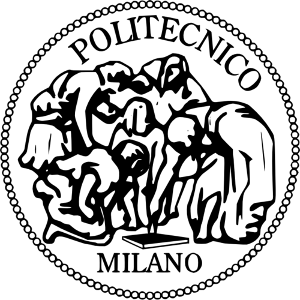
\includegraphics[width=5cm]{logo.png}

\vspace*{0.6cm}
{\Large\textsc{Politecnico di Milano}}\\
\rule{7cm}{1pt}

\vspace*{0.5cm}

Corso di Laurea Triennale in \textsc{Ingegneria Matematica}\\
Scuola di \textsc{Ingegneria Industriale e dell'Informazione}\\
\vspace*{1.3cm} 
{\LARGE\textmd{\textbf{
Sull'esistenza di soluzioni locali\\di equazioni differenziali\\\vspace*{0.2cm} alle derivate parziali
}}}

\vspace*{1.5truecm} 

{\small Tesi di}
{\large\vspace*{0.3cm}\\Alessandro Pedone}

\vspace*{1.3cm}

\begin{tabular}{@{}ll}
\small
Relatore:\\[0.5cm]
\normalsize
\quad Prof. Maurizio Grasselli & .......................................\\[1cm]
\small
Candidato:\\[0.5cm]
\normalsize
\quad Alessandro Pedone & .......................................\\
\end{tabular}
\vfill
\rule{6cm}{1pt}

\small
Sessione di Laurea Settembre 2024\\
Anno Accademico 2023/2024
\end{center} 
\clearpage
}
\blankpage

% conta con i numeri romani 
\pagenumbering{roman}

% citazione
\setlength\epigraphwidth{8cm}
\setlength\epigraphrule{0pt}
\vspace*{\fill}
\epigraph{\textit{All his life -- he had difficulty saying this, as he admitted, being always wary of too much enthusiasm -- all his life he had been waiting for such a student to come into this room. A student who would challenge him completely, who was not only capable of following the strivings of his own mind but perhaps of flying beyond them.}}{--- \textup{Alice Munro}, \textit{Too Much Happiness}}
\vspace*{\fill}
%indice
\tableofcontents

\newpage
\blankpage
%\chapter*{Sommario}
\addcontentsline{toc}{chapter}{Sommario}
Prerequisiti\\
Struttura dei capitoli e senso della trattazione: dare uno sguardo di insieme ai teoremi più importanti per la teoria locale, 
nelle forme più generali possibile, per poi dare un focus successivo alle equazioni lineari 
dove si riescono ad enunciare con efficacia condizioni sufficienti (Holmgren) e condizioni necessarie (Hörmander).\\
NOTAZIONE MULTI-INDICE\\
Derivate parziali
$$D^\alpha(u)$$
$$D^{ke_i}(u)=\frac{\partial ^ku}{\partial x_i^k}=\partial ^k_{x_i}u$$
$$k=1 \implies \partial _{x_i}u=u_{x_i}$$
Gradiente
$$Du=\nabla u=\left[u_{x_1},\ldots,u_{x_n}\right]$$
Matrice Hessiana
$$D^2u=Hu=\left[
\begin{matrix}
\nabla u_{x_1}\\
\vdots\\
\nabla u_{x_n}
\end{matrix}
\right]$$

Proprietà fondamentali
Leibniz...

varietà e serie di taylor


% ricomincia a contare con i numeri arabi
\newpage
\pagenumbering{arabic}

% rimuovi i numeri a piè di pagina
\makeatletter
\let\ps@plain\ps@empty
\makeatother

% inserisci le intestazioni per i capitoli
\pagestyle{fancy}
\renewcommand{\chaptermark}[1]{\markboth{\textit{\thechapter.\ #1}}{}}
\renewcommand{\sectionmark}[1]{\markright{\textit{\thesection.\ #1}}}
\fancyhead{} % cancella tutti i campi
\fancyhead[RO,LE]{\bfseries \thepage}
\renewcommand{\headrulewidth}{0.4pt}
\cfoot{}
\fancyhead[LO]{\rightmark}
\fancyhead[RE]{\leftmark}
\setlength{\headheight}{18pt}

%\chapter{Introduzione.}
Abbreviato CK

\section{Chi era Kowalevski?}

Sofya Vasilyevna Kovalevskaya

\textbf{Perché non Kovalevskaya}:  La stessa Kovalevskaya, per le pubblicazioni accademiche internazionali, soleva firmarsi Sophie Kowalevski

\textbf{Biografia}: background familiare, studi in germania, aiuto di Weierstrass (lezioni private e quattro tesi di dottorato), idee politiche (socialiste e radicali, sua sorella Anna le diede copies of radical journals of the time discussing Russian nihilism) e movimenti femministi, successo grazie alle tesi (I suoi risultati, tra cui il Teorema di Cauchy-Kovalevskaya, furono pubblicati nel 1875. Fu così che ottenne, prima donna in Europa, un dottorato in matematica), ritorno in russia inutile per la sua carriera accademica, in svezia dopo la morte del marito (Divenne, prima donna al mondo, professoressa di matematica, ottenendo la cattedra all'Università di Stoccolma (Högskola)), anche produzione letteraria, morte prematura a 41 anni nel 1891 di polmonite

\textbf{Nichilismo antico}: For the nihilists, science appeared to be the most effective means of helping the mass of people to a better life. Science pushed back the barriers of religion and superstition, and "proved" through the theory of evolution that (peaceful) social revolutions were the way of nature. For the early nihilists, science was virtually synonymous with truth, progress and radicalism; thus, the pursuit of a scientific career was viewed in no way as a hindrance to social activism. In fact, it was seen as a positive boost to progressive forces, an active blow against backwardness.

\textbf{Contributi}: nell'equazioni differenziali alle derivate parziali (teorema di CK) e nella meccaninca (Lagrange, Euler, and Kovalevskaya tops)

\textbf{Rappresentazione cinematografica}

Ayan Gasanovna Shakhmaliyeva è nata il 12 novembre 1932. Luogo di nascita: Baku, Azerbaijan SSR, USSR [ora Azerbaijan]. È conosciuta come regista e aiuto regista. È celebre per aver partecipato a Eto bylo u morya ... (1989), Malchishki (1970) e Dom naprotiv (1958). Morì il 27 aprile 1999. “Sofya Kovalevskaya” (1985, 3 episodi, 218 minuti, biografico, Lenfilm, OTF, colore). Gran Premio al Festival Internazionale del Film Televisivo Multiepisodio di Pianciano Terme, Italia, nel 1985.

A Hill on the Dark Side of the Moon (Swedish: Berget på månens baksida) is a 1983 Swedish drama film directed by Lennart Hjulström

\textbf{In letteratura}

\textbf{Cronologia delle dimostrazioni}
\begin{itemize}
\item
L'anno dopo la sua morte, la sua cara amica Anne Charlotte Leffler, sorella del matematico Gösta Mittag-Leffler e moglie dell'algebrista italiano Pasquale del Pezzo, le dedicò una biografia (Sonja Kovalevsky. Ciò che ho vissuto con lei e ciò che mi ha detto di sé, Ed. Albert Bonniers, Stoccolma, 1892)
\item 
Little Sparrow: A Portrait of Sophia Kovalevsky (1983), Don H. Kennedy, Ohio University Press, Athens, Ohio
\item
Beyond the Limit: The Dream of Sofya Kovalevskaya (2002) a biographical novel by mathematician and educator Joan Spicci, published by Tom Doherty Associates, LLC
\item
"Too Much Happiness" (2009), short story by Alice Munro, published in the August 2009 issue of Harper's Magazine (ispirato dal primo, infatti il racconto ripercorre gli ultimi giorni di vita di Sof'ja Kovalevskaja arricchito da reminiscenze del passato che Munro ha acquisito da lettere, diari e scritti. Munro ha potuto accedere a tali documenti tramite la moglie di Don H. Kennedy la quale è una lontana discendente di Kovalevskaja)
\end{itemize}


\chapter{Nozioni propedeutiche}
In questo capitolo vengono trattate delle nozioni fondamentali per la trattazione della teoria locale presentata.\\
Si tratta il metodo delle caratteristiche che sarà cruciale nella dimostrazione del teorema di CK anche se in una forma meno generale di quella presentata

\section{Equazioni differenziali alle derivate parziali}
\section{Superfici caratteristiche}
Cosa si intende per superficie analitica\\
Definizione di superficie caratteristica

\begin{enumerate}[i.]
\item
caso $t=0$ e calcolo di tutte le derivate (evans)
\item
caso lineare (folland)
\item
caso quasi lineare (folland)
\item
caso generale e calcolo di tutte le derivate (evans)
\item 
classificazione delle EDP
\end{enumerate}


\section{Metodo delle caratteristiche}

\begin{enumerate}[i.]
\item
caso lineare (folland)
\item
caso quasi lineare (folland)
\item
caso generale (evans)
\end{enumerate}

%\chapter{Il teorema di Cauchy-Kovalevski}
\section{Versione per EDO}
Versione per EDO
\section{Versione per EDP quasi-lineari}
Versione per EDP quasi-lineari
Rifacendoci a Evans, e quindi anche usando la notazione in esso presente, 
assumiamo che i coefficienti del sistema $B_j$ e $c$ abbiano come raggi di convergenza $r_{B_j}>0$ e $r_c>0$ 
di conseguenza per il Lemma nel capitolo 4.6.2 si osserva che affinché la maggiorazione valga è necessario 
che $r<\min\{\min_{j} \{r_{B_j}\}, r_c \}$.
Consideriamo ora la funzione $$\nu=\frac{r-s-\sqrt{(r-s)^2-2tCrmn}}{mn}$$ e ricordiamone alcune proprietà:
\begin{enumerate}[1.]

\item
E' interessante perché essa alla conclusione della dimostrazione del teorema di CK 
permette di scrivere in forma compatta la soluzione del problema maggiorante nella seguente forma: 
$$u = \nu(x_1+\ldots+x_{n-1}, t)[1,\ldots,1]^T$$

\item
Essa è analitica in un intorno dell'origine, in particolare per $t<\frac{(r-s)^2}{2Crmn}$ e di 
conseguenza anche in $B_h(0,0)$ con $h=\frac{r}{8Cmn}$.

\item
In $B_h(0,0)$ vale la condizione $s^2+m\nu ^2 (s,t)< r^2$

\item
Unendo le ultime due condizioni si ottiene che la soluzione è maggiorante in 

\end{enumerate}

\section{Versione per EDP non lineari}
Versione per EDP non lineari
Riscrivere l'equazione come un problema di evoluzione (vedi pdf)



\chapter{Esempi}

Dopo aver visto il teorema di Cauchy-Kovalevskaya in tutte le sue forme più note, si concentra ora lo sguardo su tre esempi importanti  che aiutano a inquadrare meglio il ruolo che giocano le ipotesi e che limiti ha questo teorema.

Tale discussione risulta particolarmente di rilievo, poiché per molto tempo si ritenne ragionevole pensare che un'equazione differenziale con coefficienti piuttosto regolari, come ad esempio $C^\infty$, dovesse avere almeno una soluzione. Questo, però, oltre al caso di analiticità trattato dal teorema oggetto del capitolo, in generale non accade.


\section{Esempio di Lewy}
Questo primo esempio è decisamente il più importante ed interessante tra quelli qui trattati, 
proprio perché permette di introdurre in modo più rigoroso il problema appena citato.

Nel 1957 Hans Lewy propose questo semplice controesempio, volto a mostrare come l'ipotesi di \textbf{analiticità} nel teorema di 
Cauchy-Kovalevskaya fosse cruciale, portando un caso di un operatore differenziale lineare con coefficienti analitici che necessita 
della presenza di una forzante anch'essa analitica per possedere delle soluzioni almeno $C^1$.

Ciò mostra come sia cruciale, non solo una discussione sulle condizioni sufficienti per l'esistenza di soluzioni locali, 
ma anche una sulle condizioni necessarie. Infatti Hörmander, matematico che contribuì ampiamente alla teoria delle equazioni lineari, 
rispose all'emersione di questo problema proprio con delle condizioni necessarie per l'esistenza di soluzioni locali 
(e quindi anche globali!) per equazioni lineari, le quali ispirarono poi a loro volta il lavoro di Treves e Nirenberg volto 
alla ricerca di condizioni necessarie e sufficienti.


Preliminarmente si riportano qui sotto gli enunciati di due teoremi che torneranno utili nella discussione:

\begin{namedtheorem}[Formula di Green in $\mathbb{C}$]
\hpth{
D \subseteq \mathbb{C} \text{ dominio regolare }\\
f:D \rightarrow \mathbb{C}\\
f \in H(\interior{D})
}
{\oint\limits_{\partial^+D}f(z)\,dz=2i\iint\limits_D\frac{\partial f}{\partial \overline{z}}(x+iy)\,dxdy}
\end{namedtheorem}

\begin{remark}
La definizione di dominio regolare non tornerà particolarmente utile, infatti ai fini di questa trattazione è sufficiente sapere che una qualsiasi palla chiusa è regolare (questo verrà utilizzato nella dimostrazione del teorema \ref{Lewy}). Per una formalizzazione di questo concetto si veda \cite[cap.8]{FMS}, dove è presente una trattazione dell'analogo teorema in $\mathbb{R}^2$ che va sotto il nome di ``Formule di Gauss-Green'' e ``Formula di Stokes'', di quale la generalizzazione in $\mathbb{C}$ è immediata.
\end{remark}

\begin{namedtheorem}[Principio di riflessione di Schwarz]
\hpth{
D \subseteq \mathbb{C} \text{ dominio regolare e simmetrico rispetto a } \mathbb{R}\\
D \cap\ \mathbb{R} \text{ è un intervallo }\\
f:D \rightarrow \mathbb{C}\\
f(\mathbb{R} \cap D) \subseteq \mathbb{R}\\
f \in H(\interior{D})
}
{f(\overline{z})=\overline{f(z)} \quad \forall z \in \interior{D}}
\end{namedtheorem}

\begin{remark}
La definizione di insieme simmetrico rispetto a $\mathbb{R}$ è data in modo naturale: esso deve soddisfare la condizione $z \in D \implies \overline{z} \in D$.
\end{remark}

Per entrare nel vivo dell'esempio, si definisce il seguente operatore:
$$L=D_x+iD_y-2i(x+iy)D_t$$
che soddisfa le proprietà precedentemente enunciate e il cui comportamento peculiare emerge dal teorema che si enuncia di seguito.

\begin{theorem}\label{Lewy}
\hpth{
f \text{ funzione continua a valori reali che dipende solo da } \; t\\
u\in C^1\;:\;Lu=f \text{ in un intorno dell'origine }
}
{f \text{ analitica in un intorno di } t=0}
\end{theorem}

\begin{proof}
Innanzitutto si fissa un $R>0$ tale che $\{(x,y,t): x^2+y^2<R^2,|t|<R\}$ sia contenuto nell'intorno dell'origine delle ipotesi (ovviamente questo $R$ esiste sempre) e si procede seguendo questi passi:
\begin{enumerate}[1.]
\item
Si definisce la funzione: 
\begin{equation*}
V(t,s)=\int\limits_{\gamma_r}u(x,y,t) \, dz \quad \text{con} \quad
\begin{system}
t \in (-R,R)\\
r^2=s \in [0,R^2)\\
\gamma_r=\partial^+B_r(0,0)\\
z=x+iy
\end{system}
\end{equation*}
\item
Si ricerca una relazione tra $V_s$ e $V_t$:
\begin{align*}
V&=i\iint\limits_{B_r(0,0)}(u_x+iu_y)(x,y,t) \, dx \, dy &\text{per formula di Green}\\
&=i\int_0^r \int_0^{2\pi} (u_x+iu_y)(\rho \cos \theta,\, \rho \sin \theta,\, t) \, \rho \,d\rho \, d\theta &\text{in coordinate polari}\\
V_r&=i\int_0^{2\pi} (u_x+iu_y)(\rho \cos \theta,\, \rho \sin \theta,\, t) \, r \, d\theta &\text{derivando}\\
&=\int\limits_{\gamma_r}(u_x+iu_y)(x,y,t) \, r \, \frac{dz}{z}\\
V_s&=\frac{1}{2r}V_r=\int\limits_{\gamma_r}(u_x+iu_y)(x,y,t) \, \frac{dz}{2z}\\
&=\int\limits_{\gamma_r}u_t(x,y,t) \, dz + \int\limits_{\gamma_r}f(t) \, \frac{dz}{2z} &\text{usando } Lu=f\\
&=iV_t + \pi i f(t) \numberthis \label{eq:4}
\end{align*}
\item
Si definiscono le funzioni:
\begin{align*}
F(t)&=\int_{0}^{t} f(\tau) \, d\tau\\
U(t,s)&=V(t,s)+\pi F(t)\;.
\end{align*}
e si osservano le seguenti proprietà di $U$ vista come funzione di $w=t+is$: 
\begin{itemize}
\item
si verifica che soddisfa l'equazione di Cauchy-Riemann $U_t+iU_s=2U_{\overline{z}}=0$ utilizzando la relazione \eqref{eq:4},
\item
olomorfa per $(s,t) \in (0,R^2) \times (-R,R)$ per la proprietà precedente,
\item
continua per $(s,t) \in [0,R^2) \times (-R,R)$ perché lo è $V$,
\item
$U(0,t)=\pi F(t)$ per $t\in (-R,R)$, ovvero assume valori reali sull'asse reale.
\end{itemize}
\item
Si prolunga analiticamente $U$ in un intorno dell'origine, infatti, 
date le proprietà appena osservate, valgono le ipotesi del principio di riflessione di Schwarz che ci permette 
di definire U per $s\in (-R^2,0)$ con la seguente formula: $$U(t,s)=\overline{U(t,-s)}.$$
\item
Si conclude il ragionamento notando che, se il prolungamento di $U$ è analitico in un intorno dell'origine, lo deve essere anche $U(t,0)=\pi F(t)$ e anche $f=F'$.
\end{enumerate}
\end{proof}

\textbf{Generalizzazione.} Il teorema appena trattato si presta in realtà anche a una generalizzazione interessante e l'idea è la seguente: si cerca di mostrare che, nonostante la forma caratteristica di $L$ non abbia punti singolari, è possibile scegliere una forzante $F \in C^{\infty} (\mathbb{R}^3, \mathbb{R})$ in modo tale che \textbf{ovunque} l'equazione differenziale $Lu=F$ non ammetta soluzioni.

\begin{remark}
Dati due spazi matrici $(X,d_X)$ e $(Y,d_Y)$, con la notazione $C(X,Y)$ con $k \in \mathbb{N} \cup \{\infty\}$ si indica l'insieme delle funzioni continue del tipo $h:X \rightarrow Y$. Nel caso in cui $X=\mathbb{R}^n$ e $Y=\mathbb{R}^m$ si usa la notazione $C^k(\mathbb{R}^n,\mathbb{R}^m)$ naturalmente per le funzioni $C^k$.
\end{remark}

Prima di scendere nello specifico di questa seconda parte della discussione dell'esempio di Lewy, è utile richiamare tre definizioni:
\begin{definition}
Un sottoinsieme $D$ di uno spazio topologico $X$ è denso se per ogni $ A \in X$ aperto $D \cap A \neq \emptyset $.
\end{definition}
\begin{definition}
Un sottoinsieme $E$ di uno spazio metrico è senza parte interna se $\interior{E}=\emptyset$.
\end{definition}
\begin{definition}
Uno spazio topologico viene detto ``di Baire'' se l'unione numerabile di ogni famiglia di insiemi chiusi con interno vuoto ha interno vuoto.
\end{definition}

La ragione per cui si citano questi concetti è che si è interessati a un teorema, o per meglio dire a un suo corollario, che permette di sviluppare un argomento per assurdo, nel caso si abbia a che fare con spazi metrici completi. Si riportano di seguito gli enunciati. 

\begin{namedtheorem}[Teorema della categoria di Baire]\label{Baire}
\hpthth{
(X,d) \text{ spazio metrico completo }\\
\{A_n\}_{n \in \mathbb{N}} \subseteq 2^X \text{ famiglia di insiemi aperti densi in } X\\
\{E_n\}_{n \in \mathbb{N}} \subseteq 2^X \text{ famiglia di insiemi chiusi e senza parte interna }
}
{\bigcap\limits_{n \in \mathbb{N}} A_n \text{ è denso in X }}
{\bigcup\limits_{n \in \mathbb{N}} E_n \text{ è senza parte interna }}
\end{namedtheorem}

\begin{remark}
Con questo teorema si mostra proprio come gli spazi metrici completi siano di Baire nella topologia indotta dalla metrica. Si veda \cite[cap.10]{RF} per la dimostrazione e maggiori dettagli.
\end{remark}

\begin{namedtheorem}[Corollario (argomento per assurdo di Baire)]\label{arg-Baire}
\hpth{
(X,d) \text{ spazio metrico completo }\\
\{E_n\}_{n \in \mathbb{N}} \subseteq 2^X \text{ famiglia di insiemi chiusi }\\
X=\bigcup\limits_{n \in \mathbb{N}} E_n
}
{\exists \, n \in N \text{ tale che } \interior{E_n} \neq \emptyset}
\end{namedtheorem}

\begin{remark}
Questo enunciato è la proposizione contronominale della Tesi 2 del teorema \ref{Baire} e, come è stato anticipato, può essere usato per ottenere un assurdo esibendo un spazio metrico completo uguale all'unione di una famiglia di insiemi chiusi e senza parte interna.
\end{remark}


Il secondo importante risultato di analisi funzionale, che giocherà un ruolo importante per raggiungere lo scopo dichiarato, è il teorema di Ascoli-Arzelà: un teorema ``di compattezza'', il quale sostituisce il teorema di Heine-Borel nel compito di ricerca di una sottosuccessione convergente, nel caso in cui non si abbia a che fare con spazi metrici di cui sia nota la proprietà di compattezza. In particolare verrà utilizzato per dimostrare che un insieme (di cui si capirà la struttura più avanti) è chiuso, sfruttando la proprietà di convergenza uniforme che la tesi garantisce e tenendo in considerazione che è un insieme viene detto ``chiuso'' se e solo se per ogni successione convergente completamente contenuta in esso, quest'ultima converge proprio a un elemento dell'insieme.

Per comprendere a pieno l'enunciato di tale teorema, si richiamano insieme ad esso due definizioni.
\begin{definition}
Una successione di funzioni $\{f_n:X\rightarrow\mathbb{R}\}_{n \in \mathbb{N}_0}$ si dice uniformemente limitata in $X$ se $\exists \, M\geq 0$ tale che $|f_n|\leq M$ in $X$.
\end{definition}
\begin{definition}
Una successione di funzioni $\{f_n:X\rightarrow\mathbb{R}\}_{n \in \mathbb{N}_0}$ si dice equicontinua in $X$ se $\forall \varepsilon >0 \;\, \exists \, \delta >0$ tale che $d(x,y)<\delta \implies \abs{f_n(x)-f_n(y)}<\varepsilon \quad \forall x,y \in X,\, \forall n \in \mathbb{N}_0 $.
\end{definition}
\begin{namedtheorem}[Teorema di Ascoli-Arzelà]
\hpth{
(X,d) \text{ spazio metrico completo }\\
\{f_n:X\rightarrow\mathbb{R}\}_{n \in \mathbb{N}_0} \text{ successione di funzioni }\\
\quad - \quad \text{uniformemente continua}\\
\quad - \quad \text{equilimitata}
}
{\exists \, f\in C(X,\mathbb{R}), n_k \text{ tali che } f_{n_k}\rightarrow f \text{ uniformemente }}
\end{namedtheorem}

Dopo aver inquadrato questi strumenti, è arrivato il momento di entrare nel merito discussione e lo si fa con uno schema che presenta per punti e a grandi linee il ragionamento da affrontare:
\begin{enumerate}
\item
traslare il problema del teorema \ref{Lewy} in modo da ricondursi al caso di un generico punto $(x_0,y_0,t_0)$, usando come forzante la funzione $g(x,y,t)=f(t-2xy_0+2x_0y)$ (lemma \ref{lemma-tr});
\item
costruire una funzione $S_a \in C^\infty$ per ogni $a \in l^\infty$ (lemma \ref{lemma-serie});
\item
costruire degli insiemi $E_{j,n} \subseteq l^\infty$ chiusi e senza parte interna sfruttando $S_a$ e il teorema di Ascoli-Arzelà (lemma \ref{lemma-e});
\item
concludere la dimostrazione del teorema \ref{Lewy2} utilizzando i lemmi appena citati per ricavare, con un ragionamento per assurdo, l'uguaglianza $l^\infty = \bigcup E_{j,n}$, grazie alla quale si può applicare l'argomento di Baire.
\end{enumerate}

Di seguito si dettagliano i passaggi appena elencati con enunciati e dimostrazioni.

\begin{lemma}\label{lemma-tr}
\hpth{
F \in C^\infty(\mathbb{R},\mathbb{R})\\
(x_0,y_0,t_0)\in \mathbb{R}^3\\
u\in C^1\;:\;Lu(x,y,t)=F'(t-2xy_0+2x_0y) \text{ in un intorno di } (x_0,y_0,t_0)\\
}
{F \text{ e } F' \text{ sono analitiche in un intorno di } t=t_0}
\end{lemma}

\begin{proof}
sfruttando l'invarianza dell'operatore $L$ rispetto a $$T(x,y,t)=(x+x_0,y+y_0,t+t_0+2xy_0-2x_0y),$$ ovvero la validità dell'identità (facile da verificare) $L(u \,\circ\, T)=(Lu) \circ T$, si deduce che, se $u$ è soluzione dell'equazione delle ipotesi, essa rende vera in un intorno dell'origine anche l'espressione:
\begin{equation}\label{eq:10}
L(u \circ T)(x,y,t)=f(t+t_0) \text{ con } f=F'.
\end{equation}
Chiaramente $u \circ T \in C^1$ e $g(t)=f(t+t_0)$ soddisfano le ipotesi del teorema \ref{Lewy} e quindi applicandolo alla seconda equazione la tesi è dimostrata.
\end{proof}
\begin{remark}
L'analiticità di $F$ segue dall'ultimo passaggio della dimostrazione del teorema \ref{Lewy}, tendendo in considerazione del fatto che essa è della forma $F(t)=\int_{0}^{t} f(\tau)+c$ con $c\in \mathbb{R}$.
\end{remark}
\begin{remark}
L'equazione \eqref{eq:10} vale in un intorno dell'origine poiché l'operatore $T$ rende $\mathbb{R}^3$ un gruppo, noto in generale come gruppo di Heisenberg, e agisce in questo contesto come una traslazione.
\end{remark}

\begin{lemma} \label{lemma-serie}
\hpthth{
\{(x_j,y_j,t_j)\}_{j=1}^{\infty} \text{ denso in } \mathbb{R}^3\\ \label{eq:8} \numberthis 
c_j=2^{-j}e^{-\rho_j} \text{ con } \rho_j=|x_j|+|y_j| \quad \forall j \in \mathbb{N}_0\\
a=\{a_n\}_{n=1}^{\infty} \in l^{\infty}\\
F \in C^{\infty} (\mathbb{R},\mathbb{R}) \text{ periodica e non analitica }\\
f_j(x,y,t)=F'(t+2xy_j-2x_jy)
}
{S_a=\sum_{j=1}^{\infty} a_jc_jf_j \text{ converge uniformemente in } \mathbb{R}^3}
{\text{lo stesso vale per le derivate formali } D^{\alpha}S_a=\sum_{i=1}^{\infty} a_jc_jD^{\alpha}f_j}
\end{lemma}

\begin{remark}
Naturalmente $S_a$ è una funzione $C^\infty$.
\end{remark}

\begin{proof}
Siccome $F$ è $C^\infty$ ed è periodica si definisce $M_k=\sup_t\abs{F^{(k)}(t)} \in \mathbb{R} \quad \forall k \in \mathbb{N}\, .$
E ciò permette di scrivere, per ogni $\alpha$ multi-indice e $j\in \mathbb{N}_0$, le seguenti disuguaglianze:
\begin{align*}
|a_jc_jD^{\alpha}f_j| &\leq \norm{a}_\infty \, 2^{-j} \, e^{-\rho_j} \, M_{| \alpha |+1} \, \rho_j^{| \alpha |} \\
&\leq \norm{a}_\infty \, 2^{-j} \, M_{| \alpha |+1} \left(\frac{| \alpha |}{e}\right)^{| \alpha |}& \text{ poichè } \max\limits_{x \geq 0}\frac{x^{| \alpha |}}{e^x} = \left(\frac{| \alpha |}{e}\right)^{| \alpha |} \label{eq:5}\numberthis
\end{align*}
$D^\alpha S_a$ converge totalmente, e quindi anche uniformemente, essendo che la serie $$\sum_{j=1}^{\infty} \sup\limits_{\mathbb{R}^3} |a_jc_j D^{\alpha} f_j|$$ ha un termine generale minore o uguale della parte destra della disuguaglianza \eqref{eq:5}, la cui corrispondente serie numerica è ovviamente convergente.

\end{proof}

\begin{remark}
Prima di proseguire è utile soffermarsi brevemente su due questioni:
\begin{itemize}
\item
$l^{\infty}$ è una spazio di Banach se dotato della norma: $\norm{b}_\infty=\sup_n|b_n|$ per ogni $b \in l^{\infty}$;
\item
esiste una funzione $f$ con le proprietà delle ipotesi: per esempio, la funzione $$F(x)=\sum_{n=1}^\infty\frac{\cos(n!\,x)}{(n!)^n}$$ è definita da un serie puntualmente convergente ed è $C^{\infty}(\mathbb{R},\mathbb{R})$, inoltre è periodica di periodo $2\pi$ e si può dimostrare che essa non è analitica in nessun punto $x\in\mathbb{R}$. Sopratutto per quest'ultimo aspetto si veda il problema 4 presente in \cite[cap.3]{John} per maggiori dettagli.
\end{itemize}
\end{remark}
\textbf{Notazione.} $A_{j,n} = B_{n^{-1/2}}(x_i,y_i,t_i)$ dove $(x_i,y_i,t_i)$ sono i punti nelle ipotesi del lemma \ref{lemma-serie}.
\begin{lemma}\label{lemma-e}
\hpth{
\text{Stesse ipotesi del lemma \ref{lemma-serie}}\\
\{E_{j,n}\}_{j,n \in \mathbb{N}_0} \subseteq l^{\infty} \text{ tali che } a \in E_{j,n} \; \iff \; \exists \, u \in C^1(A_{j,n}) \text{ tale che }\\
\quad - \quad Lu=S_a \text{ in } A_{j,n}\\
\quad - \quad u(x_j,y_j,t_j)=0 \numberthis \label{eq:9} \\
\quad - \quad |D^{\alpha}u| \leq n \text{ per } | \alpha | \leq 1 \text{ in } A_{j,n} \\
\quad - \quad |D^{\alpha}u(v) - D^{\alpha}u(w)| \leq n |v-w|^{1/n} \text{ per }
\begin{system}
| \alpha | = 1\\
v,w \in A_{j,n}
\end{system}
}
{\{E_{j,n}\} \text{ sono insiemi chiusi e senza parte interna}}
\end{lemma}

\begin{proof} 
si dimostrano separatamente le due proprietà:
\begin{enumerate}
\item
Per quanto riguarda la proprietà di chiusura, si vuole mostrare che se $\{a^k\}\subseteq E_{j,n}$ è tale che $a^k \xrightarrow{l^\infty} a$ allora $a \in E_{j,n}$. Ciò, a sua volta, si riduce a mostrare l'esistenza di una funzione $u$ con le proprietà in \eqref{eq:9}.

Si deduce immediatamente che $S_{a^k} \rightarrow S_a$ in modo uniforme, poiché $\abs{S_a - S_{a^k}} \leq M_1 \norm{a-a^k}$ per la \eqref{eq:5} con $\alpha = 0$. Inoltre, per le ipotesi su $a^k$ esiste una funzione $u_k$ che risolve l'equazione $Lu_k=S_{a^k}$ e che soddisfa le altre proprietà in \eqref{eq:9}. Proprio grazie a queste ultime $u_k$ soddisfa le ipotesi del teorema di Ascoli-Arzelà con $X=A_{j,n}$, quindi per una qualche $u$ vale che $u_{k_h} \rightarrow u \text{ uniformemente }$.

In particolare, sfruttando il fatto che $L$ è un operatore del primo ordine, si ricava facilmente che $Lu=S_a$ in $A_{j,n}$ poiché
\begin{align*}
Lu_{k_h}& \rightarrow Lu &\text{ uniformemente per le proprietà di } u_k\\
\lVert \quad &  &\\
S_{a^{k_h}}& \rightarrow S_a &\text{ uniformemente }
\end{align*}
e che $u$ eredita tutte le altre proprietà in \eqref{eq:9} da $u_k$ grazie alla convergenza uniforme.
 
\item
In ultimo si vuole mostrare che $\interior{E}_{j,n}=\emptyset$ ragionando per assurdo. Si suppone che esista una successione $a$ interna a $\interior{E}_{j,n}$. Definendo poi
$$\delta_j = \frac{1}{c_j} \mathds{1}_{\{j\}} \in l^\infty,$$
si osserva che esiste un $\theta \in \mathbb{R}$ abbastanza piccolo tale che $a'=a+\theta \delta_j \in E_{j,n}$.
Siano ora $u$ e $u'$ le soluzioni rispettivamente di $Lu=S_a$ e di $Lu=S_{a'}$ con le proprietà in \eqref{eq:9} e sia
$$u''=\frac{u'-u}{\theta}.$$ 
Chiaramente è vero che $u'' \in C^1$; inoltre si deduce immediatamente usando la linearità di $L$ e la definizione della serie $S$, che vale la relazione $$Lu''=S_{\delta_j}=f_j,$$ ma ciò entra in contraddizione con il lemma \ref{lemma-tr} (di cui valgono tutte le ipotesi), non essendo $F$ analitica. 
\end{enumerate}
\end{proof}

\begin{theorem}\label{Lewy2}
\hpth{
A \subseteq \mathbb{R}^3 \text{ aperto }\\
}
{
\exists \, F \in C^{\infty}(\mathbb{R}^3,\mathbb{R}) \; : \; \nexists \, u \in C^1(A,\mathbb{R}) \text{ tale che }
\begin{system}
Lu=F \text{ in } A\\
u_x,\,u_y,\,u_t \text{ soddisfano} \\
\text {la condizione di Hölder }
\end{system}
}
\end{theorem}

\begin{remark}
L'arbitrarietà di $A$ implica che questo valga per tutti gli aperti di $\mathbb{R}^3$ e quindi che $Lu=F$ non abbia soluzioni $C^1$ e con derivate prime continue secondo Hölder da nessuna parte. 
\end{remark}

\begin{remark}
La tesi implica come conseguenza naturale che non esistano nemmeno soluzioni $C^k$ per ogni $k \geq 1$, in quanto $C^k \subseteq C^1$.
\end{remark}

\begin{proof}
Si ragiona per assurdo e si conclude nei seguenti tre passi (di cui il secondo è quello che merita più attenzione).
\begin{enumerate}
\item
$E_{j,n} \subseteq l^{\infty} $ per ogni $j,n \in \mathbb{N}_0$ ovviamente.
\item
$a \in l^{\infty} \implies a \in E_{j,n}$ per qualche $j,n \in \mathbb{N}_0$ (i quali  dipendono da $a$).

Supponendo la tesi falsa, è possibile affermare che $\forall a \in l^\infty \; \exists \, A \in \mathbb{R}^3, \, u^* \in C^1(A,\mathbb{R})$ tali che si ha che $Lu^*=S_a$ e che $u^*$ ha le derivate prime continue secondo Hölder in $A$.

Si sa, inoltre, che per la densità dell'insieme dei punti in \eqref{eq:8} esiste un $(x_j,y_j,t_j) \in A$ ed essendo $A$ aperto esiste un $k$ (scelto abbastanza grande) tale per cui $A_{j,k} \subseteq A$.

Consideriamo ora la funzione $u=u^*-u^*(x_j,y_j,t_j)$, in modo che $u$ mantenga le proprietà di $u^*$, ma soddisfi al contempo la condizione $u(x_j,y_j,t_j)$ come richiesto in una della proprietà in \eqref{eq:9}.

In ultimo è chiaro che, essendo le derivate prime di $u$ continue secondo Hölder, esiste un $m$ abbastanza grande per cui valgono le condizioni rimanenti in \eqref{eq:9} con $m$ al posto del pedice $n$ e prendendo poi $n=\max\{k,m\}$ l'implicazione è dimostrata.

\item
Dai primi due passi di conclude che $$l^{\infty}=\bigcup\limits_{j,n \in \mathbb{N}_0}E_{j,n},$$ ma, quindi, per il fatto che $l^{\infty}$ è di Banach e per le proprietà degli insiemi $E_{j,n}$, valgono sia le ipotesi del corollario \ref{arg-Baire} che la negazione della tesi. Ciò è assurdo.
\end{enumerate}
\end{proof}



\section{Esempio di Kovalevskaya}

L'esempio su cui ci si concentra è dovuto a Kovalevskaya stessa ed è stato utile a suo tempo a comprendere più a fondo, in modo quanto più essenziale possibile, l'importanza, o meglio la necessità, di assumere che la superficie scelta per assegnare i dati di Cauchy sia \textbf{non-caratteristica} per l'equazione differenziale in osservazione. Inoltre costituisce un controesempio alla congettura proposta da Weierstrass, che suggeriva la possibilità di definire funzioni analitiche attraverso equazioni differenziali. Infatti tutto ciò viene citato all'interno di una lettera rivolta a Fuchs (un matematico tedesco dell'Università di Berlino) scritta da Weierstrass (che supervisionò il lavoro di ricerca di  Kovalevskaya), con cui quest'ultimo faceva richiesta per l'accettazione delle tesi di dottorato di Sofya. La lettera è riportata integralmente in \cite[app.C]{Bio}.
 
Seguendo le orme di Kowaleski, si consideri quindi il seguente problema di Cauchy per l'equazione del calore in una dimensione:
\begin{align}
\label{eq:1}
u_t-u_{xx}&=0\\ 
\label{eq:2}
u(x,0)&=\frac{1}{1+x^2} \quad \forall \, x \in \mathbb{R}
\end{align}
\begin{remark}
La condizione per $u_x$ su $\Gamma$ necessaria per completare il problema di Cauchy è già implicitamente imposta dall'equazione
\eqref{eq:2}.
\end{remark}
\begin{remark}
In realtà il dato iniziale realmente scelto da Kovalevskaya durante la sua ricerca è $\frac{1}{1-x}$, che però si è deciso di non utilizzare qui per semplicità, evitando alcuni problemi legati alla singolarità della funzione e mantenendo invariato il significato del ragionamento.
\end{remark}
L'obiettivo che ci si pone è quello di dimostrare che non ammette soluzioni analitiche in un intorno dell'origine.

\begin{enumerate}
\item
Per cominciare si osserva che in questo caso la superficie su cui sono stati assegnati i dati di Cauchy $(1.2)$ è 
$\Gamma=\left\lbrace(x,t) \in \mathbb{R}^2:t=0\right\rbrace$. Essa in ogni punto ha come versore normale $(0,1)$ ed è, quindi,
caratteristica per l'equazione \eqref{eq:1}, poiché
$$\sum_{|\alpha|=2}^{\;} a_\alpha \boldsymbol{\nu}^\alpha = a_{(2,0)}\boldsymbol{\nu}^{(2,0)} = 0.$$
\item
Per assurdo si supponga di avere una soluzione del problema $u$ analitica in un intorno dell'origine, ovvero:
$$u(x,t) = \sum_{\alpha = (\alpha_1, \alpha_2) }^{\;} c(\alpha) \, x^{\alpha_1} \, t ^{\alpha_2}, \quad
 c(\alpha) = \frac{D^\alpha u(0,0)}{\alpha!}$$
dove $|(x,t)|<r$ per qualche $r>0$.
\item
Si calcolano i valori dei coefficienti $c(2n,0)$ $\forall n \in \mathbb{N}$.\\
Per fare questo si sviluppa in serie di potenze centrata nell'origine la funzione del problema di Cauchy:
$$\frac{1}{1+x^2} = \frac{d}{dx}\arctan(x) = \frac{d}{dx}\sum_{n=0}^{\infty}\frac{(-1)^n}{2n+1} \, x^{2n+1} 
= \sum_{n=0}^{\infty}(-1)^n \, x^{2n} \quad \forall x \in \mathbb{R}.$$
Da questa serie si ottengono le seguenti relazioni:
\begin{align*}
D_x^{2n}u(0,0) &= \frac{d^{2n}}{dx^{2n}} \left. \frac{1}{1+x^2}\right|_{x=0} = (-1)^n (2n)!\\
D_x^{2n+1}u(0,0) &= \frac{d^{2n+1}}{dx^{2n+1}} \left. \frac{1}{1+x^2} \right|_{x=0} = 0
\end{align*} 
dalle quali si ricava: $c(2n,0)=(-1)^n$ e $c(2n+1,0)=0$.
\item
Si calcolano i valori dei coefficienti $c(2n,n)$ e si dimostra che  $c(2n,n) \xrightarrow{n\rightarrow\infty} +\infty$.\\
A questo scopo, invece, si sfrutta l'equazione $(1.1)$ per ottenere la seguente relazione tra i coefficienti:
\begin{equation} 
\label{eq:3}
c(\alpha_1,\alpha_2+1) = \frac{(\alpha_1+2)(\alpha_1+1)}{(\alpha_2+1)} \, c(\alpha_1+2,\alpha_2).
\end{equation}
E si utilizza, quindi, quest'ultima come segue:
\begin{align*}
c(2n,n) &= \frac{(2n+2)(2n+1)}{n} \, c(2n+2,n-1)   &\eqref{eq:3}\quad\text{con} \quad 
\begin{system}
\alpha_1=2n\\
\alpha_2+1=n
\end{system}\\
 &= \ldots = \frac{(2n+2n)\cdots(2n+1)}{n!} \, c(2n+2n,0) &\text{\quad iterando su } n\\
 &= \frac{(4n)!}{(2n)! \, n!} (-1)^{2n} \\
 &\sim \frac{1}{\sqrt{\pi n}}\left(\frac{64n}{e}\right)^n \xrightarrow{n\rightarrow\infty} +\infty  &\text{per la formula di Stirling}
\end{align*}
\item
Si completa il ragionamento in modo immediato osservando che 
$c(2n,n) \, x^{2n} \, t ^{n}\xrightarrow{n\rightarrow\infty} +\infty$ $\forall (x,t) \neq (0,0)$, 
infatti ciò implica direttamente che la serie di potenze non converge in ogni punto diverso dall'origine e questo è assurdo.
\end{enumerate}

\section{Esempio di Hadamard}
L'esempio che si propone ora, dovuto ad Hadamard (1932), aiuta a capire un limite importante del teorema di Cauchy-Kovalevskaya, ovvero il fatto che esso non fornisca alcun controllo sulla \textbf{relazione} tra i dati di Cauchy e la forma della soluzione analitica, la quale potrebbe risultare instabile.

Per osservare ciò si considera il seguente problema di Cauchy per l'equazione di Laplace in due dimensioni al variare di $n$:
\begin{align*}
u_{xx}+u_{yy}&=0\\
u(x,0)&=0 \numberthis \label{eq:6}\\ 
u_y(x,0)&=n\sin(nx)e^{-\sqrt{n}} \quad \text{con} \quad n\in\mathbb{N}
\end{align*}


L'obiettivo che ci si pone in questo caso è quello di mostrare come al crescere di $n$ 
si verifica un blow-up della soluzione $u_n$ del problema di Cauchy \eqref{eq:6}.
\begin{enumerate}[1.]
\item
Il problema, come nell'esempio precedente, è assegnato su $\Gamma=\left\lbrace(x,y) \in \mathbb{R}^2:y=0\right\rbrace$, che è naturalmente una superficie non caratteristica per l'equazione di Laplace (si noti infatti che essa è ellittica).
\item
E' facile verificare che la funzione $u_n(x,y)=\sin(nx)\sinh(ny)e^{-\sqrt{n}}$ soddisfa il problema di Cauchy e che essa è analitica, per questo è anche l'unica possibile con quest'ultima proprietà.
\item
Si osserva, infine, come $\sinh(ny)e^{-\sqrt{n}}\xrightarrow{n\rightarrow\infty} \infty$.
\end{enumerate}
Come conclusione di questa discussione è interessante osservare anche come la soluzione non dipenda con continuità dai dati. 
Infatti, considerando il problema di Cauchy per ${n=\infty}$, ovvero con dati $u(x,0)=u_y(x,0)=0$, si nota immediatamente che l'unica soluzione analitica è $u\equiv0$, la quale è profondamente diversa dal comportamento asintotico di $u_n$.



%\chapter{Versione alternative}
%\chapter{Teorema di Holmgren}

% BIBLIOGRAFIA
% PER FARLA FUNZIONARE: eseguire latex-bibtex-latex-latex
\addcontentsline{toc}{chapter}{Bibliografia}
\nocite{*} % Inserire nella bibliografia anche le fonti non citate esplicitamente nel testo
\bibliographystyle{alpha} % We choose the "plain" reference style
\bibliography{bibliografia} % Entries are in the refs.bib file

\end{document}